\documentclass[a4paper,xelatex,ja=standard,jafont=hiragino-pron, 10pt]{bxjsarticle}

\usepackage{xltxtra}
\XeTeXlinebreaklocale "ja"

\usepackage{amsmath, amssymb, mathrsfs}
\usepackage[dviout]{}
\usepackage{fancyvrb, xcolor}
\usepackage{listings}

% \topmargin = 0mm
% \oddsidemargin = 5mm
% \textwidth = 152mm
% \textheight = 240mm

\renewcommand{\thesection}{問\arabic{section}}
\renewcommand{\thesubsection}{(\arabic{subsection})}
\renewcommand{\thesubsubsection}{(\arabic{subsection}.\arabic{subsubsection})}

\title{データ解析レポート課題・第一}
\author{14\_01043 伊澤 侑祐}
\date{}

\begin{document}
\maketitle
\section{計算問題}
\subsection{}
まず、$k$を固定する。二乗誤差

\begin{eqnarray}
  E(a) &=& \frac{1}{n} \sum_{i = 1}^n (Y_i - f(x_i, a))^2 \nonumber \\
       &=& \frac{1}{n} \sum_{i = 1}^n (Y_i - \sum_{k = 1}^K a_k e_k(x))^2
\end{eqnarray}

を$a_k$で微分し、極値条件を解く。

\begin{eqnarray}
  &&\frac{\partial E}{\partial a_k}
    = \frac{2}{n} \sum_{i = 0}^n (Y_i - a_ke_k(x)) \cdot e_k(x) = 0 \nonumber \\
    &\Longleftrightarrow& \, \sum_{i=1}^n Y_i e_k(x) - n a_k = 0 \nonumber \\
    &\Longleftrightarrow& \, a^*_k = \frac{1}{n} \sum_{i=1}^n Y_i e_k(x)
    \label{ans-1-before}
\end{eqnarray}

よって求める答えは(\ref{ans-1-before})より

\begin{equation}
  a^* = \left\{ \left(\frac{1}{n} \sum_{i=1}^n Y_i e_k(x)\right)_k \right\}
\end{equation}

である。

\subsection{}
平均を$\mathscr{E}(\cdot)$で表す。$\mathscr{E}(Y_i) = 0$を用いて、

\begin{eqnarray}
  \mathscr{E}(a^*)
    &=& \mathscr{E} \left(\frac{1}{n}\sum_{i=0}^n Y_i e_k (x) \right) \nonumber \\
    &=& 0
\end{eqnarray}

となる。
\subsection{}
まず、一般に$(k, l)$成分の場合の共分散を考える。$i$成分の期待値を$\mu_i$と置くと、

\begin{eqnarray}
  \sigma_{i, j}
    &=& \mathscr{E}
      \left(
        \left(a^*_k - \mu_i\right)
        \left(a^*_l - \mu_l\right)
      \right) \nonumber \\
    &=& \mathscr{E}\left(a^*_k \cdot a^*_l \right) \nonumber \\
    &=& \mathscr{E}
      \left(
        \left(\frac{1}{n} \sum_{i = 1}^n Y_i e_k (x_i)\right)
        \left(\frac{1}{n} \sum_{i = 1}^n Y_i e_l (x_i)\right)
      \right) \nonumber \\
    &=& \frac{1}{n^2} \mathscr{E}
      \left(
        \sum_{i, j = 1}^n Y_i Y_j e_k(x_i) e_l(x_j)
      \right) \label{var_ea_1}
\end{eqnarray}

となる。ここで、$\mathscr{E}(Y_i) = 0, \sqrt{\mathscr{E}(Y_i^2) - (E(Y_i))^2} = 1$, そして$Y_i$が独立であることより、

\begin{eqnarray}
  \mathscr{E}\left(
    \sum_{i, j = 1}^n Y_i Y_j e_k(x_i) e_l(x_j)
  \right)
    &=& \sum_{i, j = 1}^n \mathscr{E}(Y_i)\mathscr{E}(Y_j) \sum_{i, j = 1}^n e_k(x_i) e_l(x_j) \nonumber \\
    &=& \begin{cases}
      \sum_{i = 1}^n \mathscr{E}\left(Y_i^2\right)e_k(x_i) e_l(x_i) & (i = j) \\
      0  & (i \neq j)
    \end{cases} \nonumber \\
    &=& \begin{cases}
      n & (i = j) \\
      0 & (i \neq j)
    \end{cases} \label{var_ea_2}
\end{eqnarray}

となる。したがって、求める分散共分散行列 $\Sigma$ は、(\ref{var_ea_1})と(\ref{var_ea_2})より

\begin{equation}
  \Sigma = \frac{1}{n}\left(
    \begin{array}{cccc}
      1 & 0 & \ldots & 0 \\
      0 & 1 & \ldots & 0 \\
      \vdots & \vdots & \ddots & \vdots \\
      0 & 0 & \ldots & 1
    \end{array}
  \right)
\end{equation}

と求まる。

\subsection{}
$E(a^*)$の平均値$\mathscr{E}(E(a^*))$を求めると、次のようになる。

\begin{eqnarray}
  \mathscr{E}\left(E(a^*)\right)
    &=& \mathscr{E}\left(\frac{1}{n}
      \sum_{i=1}^n
        \left(
          Y_i - \frac{1}{n}\sum_{k=1}^K Y_i e_k(x_i) e_k(x_i)
        \right)^2\right) \nonumber \\
    &=& \mathscr{E}\left(\frac{1}{n} \sum_{i=1}^n
      \left(
        Y_i^2 - \frac{2}{n} \left(
          \sum_{k=1}^K Y_i^2 e_k(x_i) e_k(x_i)
        \right) + \left(
          \frac{1}{n} \sum_{k=1}^K Y_i e_k(x_i) e_k(x_i)
        \right)^2\right)
      \right) \nonumber \\
    &=& \frac{1}{n} \sum_{i=1}^n \mathscr{E} \left(Y_i^2\right) -
      \frac{2K}{n} \sum_{i=1}^n \mathscr{E} \left(Y_i^2\right) +
      \frac{1}{n}
        \sum_{k=1}^K \sum_{i=1}^n
          \left(
            \frac{1}{n}e_k(x_i)e_k(x_i)
          \right)^2  \mathscr{E}(Y_i^2) \nonumber \\
      &=& 1 - \frac{2K}{n} + \frac{K}{n} \nonumber \\
      &=& 1 - \frac{K}{n}
\end{eqnarray}
\subsection{}

\begin{equation}
  \mathscr{A} = \frac{1}{n} \int_{- \infty}^{\infty}\sum_{i=1}^n \left(
    y - f(x_i, a^*)
  \right)^2 q(y) dy
\end{equation}

とおく。まず、$\mathscr{A}$を計算する。

\begin{equation}
  \begin{split}
    \int_{-\infty}^{\infty}q(y)dy = 1, \quad
    \int_{-\infty}^{\infty}yq(y)dy = 0, \quad
    \int_{-\infty}^{\infty}y^2q(y)dy = 1
  \end{split}
\end{equation}

であることを用いて、以下のようになる。

\begin{eqnarray}
  \begin{split}
    \mathscr{A}
      &= \frac{1}{n} \sum_{i=1}^n \int_{-\infty}^{\infty} \left(
        y^2 - \frac{2}{n} \sum_{k=1}^K y Y_i e_k(x_i) e_k(x_i) +
        \left(
          \frac{1}{n} \sum_{k=1}^K Y_i e_k(x_i) e_k(x_i)
        \right)^2
      \right) q(y) dy \nonumber \\
      &= \frac{1}{n} \sum_{k=1}^n \int_{-\infty}^{\infty} y^2 q(y) dy \\
      &\qquad - \frac{2}{n^2} \sum_{k=1}^K \sum_{i=1}^n \int_{-\infty}^{\infty} y Y_i e_k(x_i) e_k(x_i) q(y) dy
      + \frac{1}{n^3} \sum_{k=1}^K \sum_{i=1}^n Y_i^2 \left(
        e_k(x_i) e_k(x_i)
      \right)^2 \cdot \int_{-\infty}^{\infty} yq(y) dy \nonumber \\
    &= \frac{1}{n} \cdot n \cdot 1 - \frac{2}{n^2} \sum_{k=1}^K \sum_{i=1}^n
      Y_i^2 e_k(x_i) e_k(x_i) \cdot \int_{-\infty}^{\infty} y q(y) dy
      + \frac{1}{n} \sum_{k=1}^K \sum_{i=1}^n Y_i^2 \left(
        \frac{1}{n}e_k(x_i)e_k(x_i)
      \right)^2 \nonumber \\
    &= 1 + \frac{1}{n} \sum_{k=1}^K \sum_{i=1}^n Y_i^2 \left(
      \frac{1}{n}e_k(x_i)e_k(x_i)
    \right)^2
  \end{split}
\end{eqnarray}

よって、$\mathscr{A}$の期待値は、

\begin{eqnarray}
  \mathscr{E}(\mathscr{A})
    &=& 1 + \frac{1}{n} \sum_{k=1}^K \sum_{i=1}^n \mathscr{E}(Y_i^2) \left(
      \frac{1}{n}e_k(x_i)e_k(x_i)
    \right)^2 \nonumber \\
    &=& 1 + \frac{K}{n}
\end{eqnarray}

となる。

\newpage
\section{応用問題}

\subsection{}
「市町村2012estat.csv」に対し、回帰分析、主成分分析とクラスタ分析を用いて解析を行った。
次の環境で解析した。

\begin{itemize}
  \item macOS Sierra 10.12.2
  \item Python 3.5.2
  \item numpy, scipy, pandas, scikit-learn, matplotlib
\end{itemize}

\subsubsection{回帰分析}

\paragraph{15歳から64歳までの人口総数と転出者数の関係}

まず、15歳から64歳までの人口総数(中間人口総数)と転出者数の関係性を調べるため、この二者に対して

\begin{equation}
  (\mbox{転出者数}) = a \cdot (\mbox{中間人口総数}) + b
\end{equation}

という仮設を立て、回帰分析を行った。その結果、次のようなグラフを得た。

\begin{figure}[ht]
  \centering
  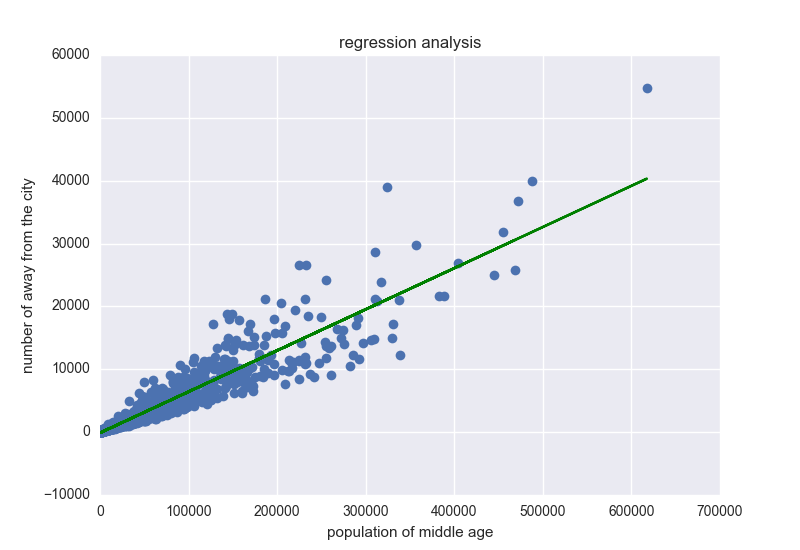
\includegraphics[clip, width=10.0cm]{../data/picture/regression_ma.png}
  \caption{15歳から64歳までの人口総数と転出者}
  \label{reg_ma}
\end{figure}

また、pandasのols関数で生成したモデルは次のようになった。

\begin{lstlisting}[
  backgroundcolor=\color{yellow},
  basicstyle=\ttfamily,
  frame=single,
  caption=モデル1]
Formula: Y ~ <x> + <intercept>

Number of Observations:         1870
Number of Degrees of Freedom:   2

R-squared:         0.8835
Adj R-squared:     0.8834

Rmse:           1505.4458

F-stat (1, 1868): 14160.3938, p-value:     0.0000

Degrees of Freedom: model 1, resid 1868

------------------Summary of Estimated Coefficients------------------------
Variable       Coef    Std Err     t-stat    p-value    CI 2.5%   CI 97.5%
---------------------------------------------------------------------------
        x     0.0655     0.0006     119.00     0.0000     0.0644     0.0666
intercept  -116.7771    41.7843      -2.79     0.0052  -198.6743   -34.8800
\end{lstlisting}

今回の場合、決定係数が0.8835とあり、このモデルで88 $\%$ 以上説明できているということになる。
また、F値が十分に大きく(14160.3938)、p値も0.0000と99$\%$以上妥当であるといえる。
さらに、係数$a$(上の表における$x$)と$b$(上の表におけるintercept)の優位確率はそれぞれ0.0000と0.0052であるため、
両方の値は妥当であるといえる。ゆえに、この仮設は妥当であると判断できる。

\paragraph{65歳以上の総人口と離婚件数の関係}

さらに、65歳以上の総人口(老年人口数)と離婚件数の関係について、

\begin{equation}
  (\mbox{離婚件数}) = a \cdot (\mbox{老年人口数}) + b
\end{equation}

という仮設を立て、回帰分析を行った。その結果、次のようなグラフを得た。

\begin{figure}[ht]
  \centering
  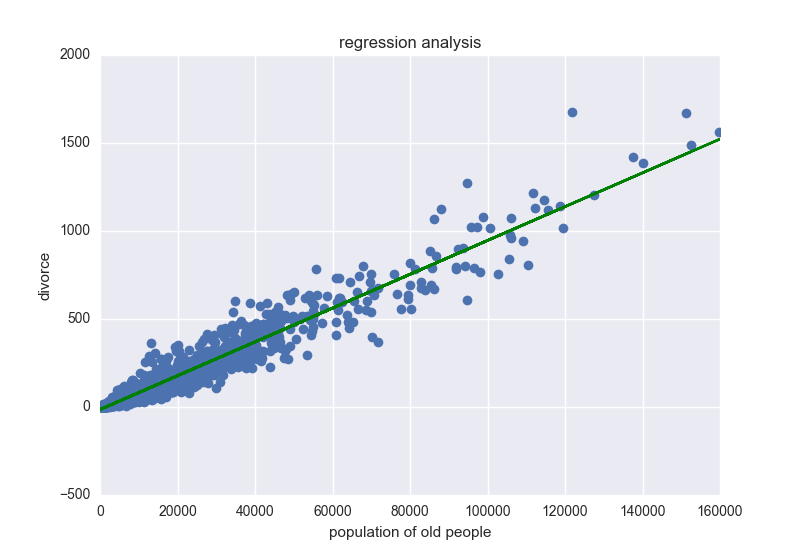
\includegraphics[clip, width=10.0cm]{../data/picture/regression_od.png}
  \caption{}
  \label{}
\end{figure}

また、pandasのols関数で生成したモデルは次のようになった。

\begin{lstlisting}[
  backgroundcolor=\color{yellow},
  basicstyle=\ttfamily,
  frame=single,
  caption=モデル2]
Formula: Y ~ <x> + <intercept>

Number of Observations:         1870
Number of Degrees of Freedom:   2

R-squared:         0.9359
Adj R-squared:     0.9359

Rmse:             51.1998

F-stat (1, 1868): 27277.3908, p-value:     0.0000

Degrees of Freedom: model 1, resid 1868

-----------------Summary of Estimated Coefficients------------------------
Variable       Coef    Std Err     t-stat    p-value    CI 2.5%   CI 97.5%
--------------------------------------------------------------------------
        x     0.0096     0.0001     165.16     0.0000     0.0095     0.0097
intercept   -14.4010     1.4768      -9.75     0.0000   -17.2956   -11.5064
\end{lstlisting}

今回の場合、決定係数が0.9359とあり、このモデルで93$\%$以上説明できているということになる。
また、F値が十分に大きく(27277.3908)、p値も0.0000と99$\%$以上妥当であるといえる。
さらに、係数$a$(上の表における$x$)と$b$(上の表におけるintercept)の優位確率はそれぞれ0.0000と0.0000であるため、
両方の値は妥当であるといえる。ゆえに、この仮設は妥当であると判断できる。

\subsubsection{主成分分析}


\end{document}
